\chapter{Results}

\section{Poisson Equation}
\label{sec:poisson_equation}

Given a region $\Omega \subset \R^d$, with $d \in \N$ and bounded by the boundary $\partial\Omega$, the generic heat equation with internal heat generation~\cite{Brezis:functional_analysis_book}, at steady state, is described by the Poisson Equation which is defined by the following Partial Differential Equation (PDE):
\begin{equation}
	\label{eqn:Poisson_equation}
	\begin{cases}
		- \Delta u(\vec{x}) = q(\vec{x})														 &  \text{in $\Omega$}							\\
		\mathcal{B} u(\vec{x}) = g(\vec{x})  													 &  \text{on $\partial\Omega$}
	\end{cases}
\end{equation}
where $\Delta$ indicates the Laplacian operator, $\mathcal{B}$ is the (possibly differential) linear operator that enforce the boundary conditions (BCs) and $q$ and $g$ are known functions.
The Poisson equation is a well-known example of a PDE that can be effectively addressed using meshless techniques, such as the RBF-FD approach detailed in this work.

We decided to evaluate the results of the adjoint method applied to RBF-FD method on the aforementioned equation due to both its wide range of applications in different areas	(e.g. electrostatic, chemistry, gravitation and others) and the simplicity of its analytical manipulation.

%\medskip
%In particular for this thesis and to obtain the results presented in this chapter we implemented RBF-FD method as follow:
%\begin{itemize}
%%TODO: 	\item consider domains $\Omega \subset \R^{d}$ with $d=1,3$;  Da spostare nell'intro ai results
%	\item use RBFs augmented with polynomial terms as basis functions $B_k$ to approximate the solution $u$ in a similar way to what has been done in~\cite{Liu:Intro_to_meshfree_methods}; 
%	\item formulate the problem in its strong form, so we will use the collocation technique in combination with the Weighted Residual Method.
%\end{itemize}
%thus we will apply the RBF-generated Finite Differences (RBF-FD)~\cite{Fornberg:RBF-FD_1, Fornberg:RBF-FD_2} to solve~\eqref{eqn:Poisson_equation} in one and three dimensional physics domain.
% "Collocation methods with Weighted Residual Methods" Cioè prima hai citato i collocation, ma i weighted residual da dove saltano fuori?? Da spiegare meglio/togliere??
%
%Mono dimensional physics domain are used to gain confidence with the techniques explained while three dimensional  domain are used for their application in real case problems as those faced at Esteco. $2$D cases, instead, have been skipped in the analysis since they would only be used to bridge the 2 previous scenarios and therefore would have had no practical utility.
%
%RBFs are used for scattered data interpolation both for their physical foundation[overview 20, Hardy 1990] and for their profitable use in applications like meteorology, turbulence analysis and neural network~\cite{Chen:meshless_overview_after_20_years}
%
%Finally, collocation technique is employed because thanks to its ability to discretize the Boundary Value problem~\eqref{eqn:Poisson_equation} expressed in strong form leads to a real fully meshless approach~\cite{Miotti:RBF_in_depth}.


\section{1D case}

In this case $d=1$. The physical domain is simply a segment and its boundary consists on its two endpoints that we indicate with $a$ and $b$, both belonging to $\R$. Therefore we have $\Omega =~]a,b[$ and $\partial\Omega = \Set{a, b}$.
For the remaining portion of the boundary value problem we define $q(x) = - \omega^2 \sin(x)$ and we impose the following Dirichlet BCs: $u(a)=q(a)$ and $u(b)=q(b)$. Fixing the values $\omega=1$, $a=0$ and $b=\pi$ allows to rewrite the Poisson equation reported in~\eqref{eqn:Poisson_equation} as
\begin{equation}
	\label{eqn:Poisson_equation_1D}
	\begin{cases}
		- \Delta u(\vec{x}) = - \sin(x)  &  \text{in $]a,b[$}  \\
		u(a) &= 0  \\
		u(b) &= 0
	\end{cases}
\end{equation}
In order to find an approximated solution to the problem~\eqref{eqn:Poisson_equation_1D} we employ the RBF-FD method parametrized as follow:
\begin{itemize}
	\item $N=41$ evenly spaced nodes are used for domain discretization: $N_I=39$ are placed in $\Omega$ and the other $N_B=2$ are placed repsectivelly in $a$ and $b$;
	\item $\varphi(r) = r^3$ Polyharmonic function is used as basic function to define the RBF interpolant;
	\item $P=2$ is the degree of its polynomial augmentation;
	\item $m=7$ is the number of nodes which constitute a single stencil;
\end{itemize}
As done previously we indicate with $\vec{u}_I$ the vector obtained by solving the system~\eqref{eqn:compact_discretized_PDE} derived from RBF-FD discretization.
%TODO: Sposta il vincolo dopo la cost function
The discretized version of equation~\eqref{eqn:Poisson_equation_1D} will be the constraints during the optimization

\smallskip
The design optimization problem, related to segment $[a,b]$, that we want to solve is the minimization of the following cost function:
\begin{equation}
	J(\vec{u}_I, b) = \frac{1}{2} \frac{b}{N-1} \left( \sum_{i=2}^{40} u(x_i) - E \right)^2
\end{equation}
where $E\in\R$ is a parameter set by us with a value of $2.5$ imposed and $l=b$ is the single design variable. This particular configuration of the design variable means that in order to meet the objective we are allowed to vary the length of the segment $[a,b]$.
%$\vec{u}_I$ is the result of the simulation performed through the RBF-FD solver and
%We remind that the discretized version of Equation~\eqref{eqn:Poisson_equation_1D} will be a constraint during the optimization.

\smallskip
The results after $30$ steps in the optimization procedure are shown in figure~\ref{fig:opt_results_1D}.

\begin{figure}
	\centering
	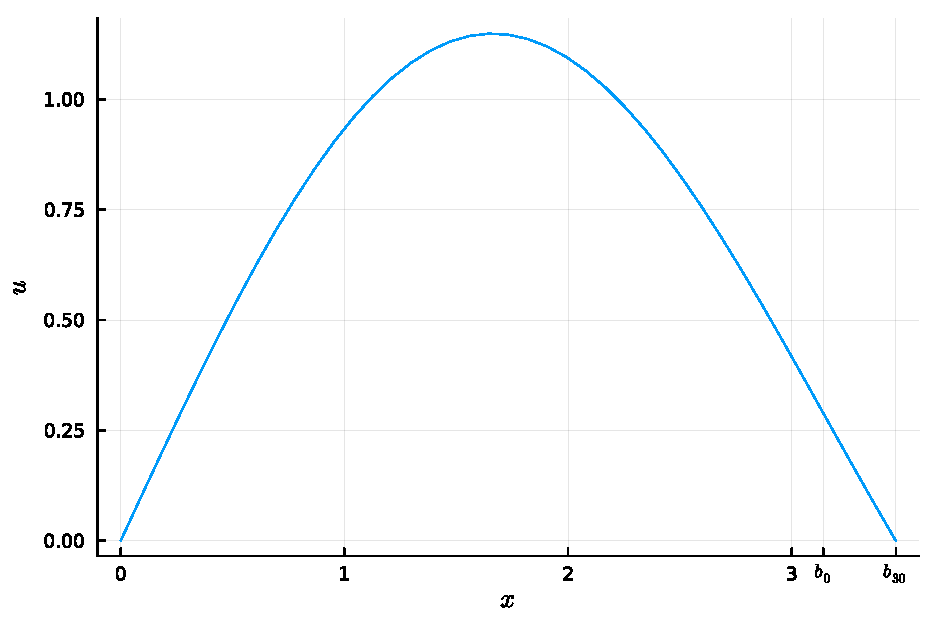
\includegraphics[width=.75\textwidth]{img/uOpt_vs_x_1D.pdf}
	\caption{discretized approximated solution obtained solving~\eqref{eqn:Poisson_equation_1D} via RBF-FD at the end of the design optimization. $b_0$ and $b_{30}$ indicate respectively the intial and the final position of the $b$ endpoint}
	\label{fig:opt_results_1D}
\end{figure}

while in figure~\ref{fig:opt_history_1D} are shown the dynamic of the cost function and of its gradient respect the design variable $b$.

\begin{figure}
	\centering
	\subfloat[][\emph{Cost function values}]
		{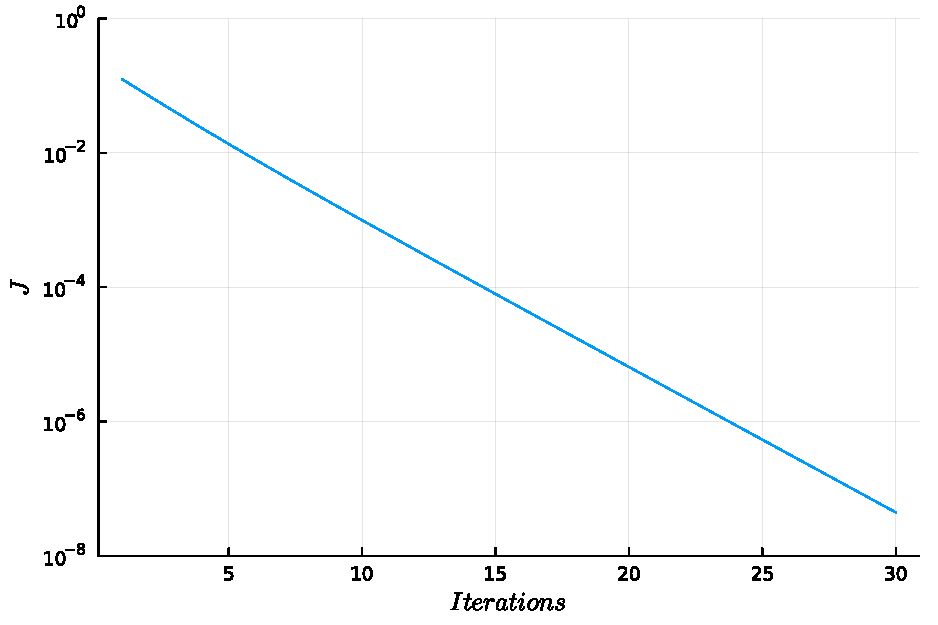
\includegraphics[width=.45\textwidth]{img/cost_vs_iter_1D.pdf}} \quad
	\subfloat[][\emph{Cost function gradient values}]
		{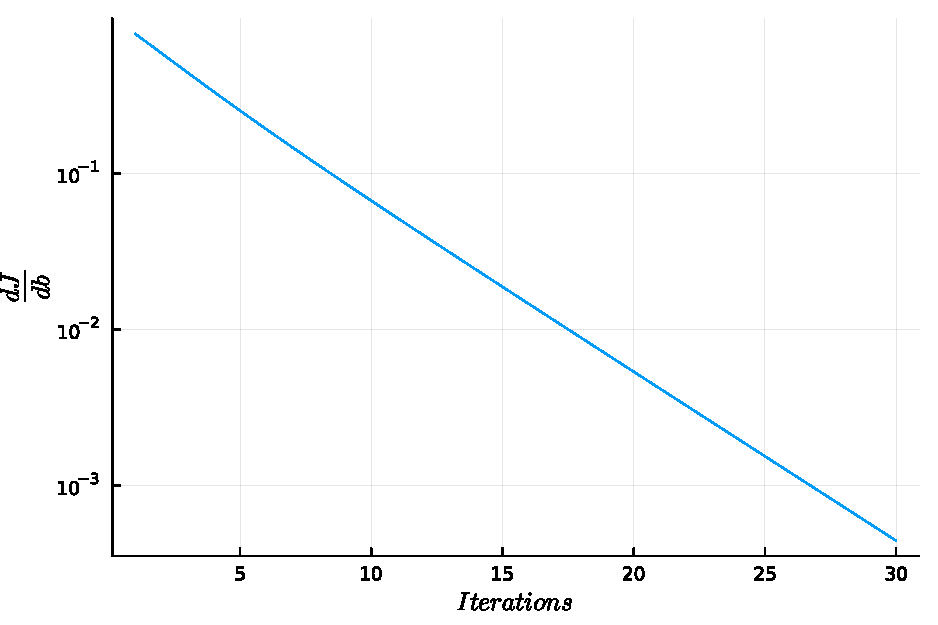
\includegraphics[width=.45\textwidth]{img/costGrad_vs_iter_1D.pdf}}
	\caption{Trajectories of the cost function and its gradient throughout the optimization process. The ordinates are on a logarithmic scale}
	\label{fig:opt_history_1D}
\end{figure}



\section{3D case}

Now we have $d=3$.
In this case the geometry is defined through a \verb|.stl| file which is an approximation of the geometry surface as a triangulated mesh. Each of these triangles will consist of three vertices and to modify the shape of the geometry we are allowed to move the position of a subset of the vertices defined in the \verb*|.stl| file; in particular we are only allowed to alter their height. The physical domain domain is defined by